\documentclass[12pt,a4paper]{report}
\usepackage[utf8]{inputenc}
\usepackage{amsmath}
\usepackage{amsfonts}
\usepackage{amssymb}
\usepackage{amsthm}
\usepackage{hyperref}

\usepackage{mathrsfs}

\usepackage{multicol}
\usepackage{fancyhdr}
\usepackage[inline]{enumitem}
\usepackage{tikz}
\usepackage{tikz-cd}
\usetikzlibrary{calc}
\usetikzlibrary{shapes.geometric}
\usetikzlibrary{positioning}
\usepackage[margin=0.5in]{geometry}
\usepackage{xcolor}

\hypersetup{
    colorlinks=true,
    linkcolor=blue,
    filecolor=magenta,      
    urlcolor=cyan,
    pdftitle={Tensors},
    pdfpagemode=FullScreen,
    }

%\urlstyle{same}

\newcommand{\CLASSNAME}{Math 5050 -- Special Topics: Manifolds}
\newcommand{\STUDENTNAME}{Paul Carmody}
\newcommand{\ASSIGNMENT}{Section 11: The Rank of a Smooth Map }
\newcommand{\DUEDATE}{July 2, 2025}
\newcommand{\PROFESSOR}{Professor Berchenko-Kogan}
\newcommand{\SEMESTER}{Fall 2025}
\newcommand{\SCHEDULE}{TBD}
\newcommand{\ROOM}{Remote}

\newcommand{\MMN}{M_{m\times n}}
\newcommand{\FF}{\mathcal{F}}

\pagestyle{fancy}
\fancyhf{}
\chead{ \fancyplain{}{\CLASSNAME} }
%\chead{ \fancyplain{}{\STUDENTNAME} }
\rhead{\thepage}
\newcommand{\LET}{\text{Let }}
%\newcommand{\IF}{\text{if }}
\newcommand{\AND}{\text{ and }}
\newcommand{\OR}{\text{ or }}
\newcommand{\FORSOME}{\text{ for some }}
\newcommand{\FORALL}{\text{ for all }}
\newcommand{\WHERE}{\text{ where }}
\newcommand{\WTS}{\text{ WTS }}
\newcommand{\WLOG}{\text{ WLOG }}
\newcommand{\BS}{\backslash}
\newcommand{\DEFINE}[1]{\textbf{\emph{#1}}}
\newcommand{\IF}{$(\Rightarrow)$}
\newcommand{\ONLYIF}{$(\Leftarrow)$}
\newcommand{\ITH}{\textsuperscript{th} }
\newcommand{\FST}{\textsuperscript{st} }
\newcommand{\SND}{\textsuperscript{nd} }
\newcommand{\TRD}{\textsuperscript{rd} }
\newcommand{\INV}{\textsuperscript{-1} }

\newcommand{\XXX}{\mathfrak{X}}
\newcommand{\MMM}{\mathfrak{M}}
%\newcommand{\????}{\textfrak{A}}
%\newcommand{\????}{\textgoth{A}}
%\newcommand{\????}{\textswab{A}}

\DeclareMathOperator{\DER}{Der}
\DeclareMathOperator{\SGN}{sgn}

%%%%%%%
% derivatives
%%%%%%%

\newcommand{\PART}[2]{\frac{\partial #1}{\partial #2}}
\newcommand{\SPART}[2]{\frac{\partial^2 #1}{\partial #2^2}}
\newcommand{\DERIV}[2]{\frac{d #1}{d #2}}
\newcommand{\LAPLACIAN}[1]{\frac{\partial^2 #1}{\partial x^2} + \frac{\partial^2 #1}{\partial y^2}}

%%%%%%%
% sum, product, union, intersections
%%%%%%%

\newcommand{\SUM}[2]{\underset{#1}{\overset{#2}{\sum}}}
\newcommand{\PROD}[2]{\underset{#1}{\overset{#2}{\prod}}}
\newcommand{\UNION}[2]{\underset{#1}{\overset{#2}{\bigcup}}}
\newcommand{\INTERSECT}[2]{\underset{#1}{\overset{#2}{\bigcap}}}
\newcommand{\FSUM}{\SUM{n=-\infty}{\infty}}
       

%%%%%%%
% supremum and infimum
%%%%%%%

\newcommand{\SUP}[1]{\underset{#1}\sup \,}
\newcommand{\INF}[1]{\underset{#1}\inf \,}
\newcommand{\MAX}[1]{\underset{#1}\max \,}
\newcommand{\MIN}[1]{\underset{#1}\min \,}

%%%%%%%
% infinite sums, limits
%%%%%%%

\newcommand{\SUMK}{\SUM{k=1}{\infty}}
\newcommand{\SUMN}{\SUM{n=1}{\infty}}
\newcommand{\SUMKZ}{\SUM{k=0}{\infty}}
\newcommand{\LIM}[1]{\underset{#1}\lim\,}
\newcommand{\IWOB}[1]{\LIM{#1 \to \infty}}
\newcommand{\LIMK}{\IWOB{k}}
\newcommand{\LIMN}{\IWOB{n}}
\newcommand{\LIMX}{\IWOB{x}}
\newcommand{\NIWOB}{\LIM{n \to \infty}}
\newcommand{\LIMSUPK}{\underset{k\to\infty}\limsup \,}
\newcommand{\LIMSUPN}{\underset{n\to\infty}\limsup \,}
\newcommand{\LIMINFK}{\underset{k\to\infty}\liminf \,}
\newcommand{\LIMINFN}{\underset{n\to\infty}\liminf \,}
\newcommand{\ROOTRULE}[1]{\LIMSUPK \BARS{#1}^{1/k}}

\newcommand{\CUPK}{\bigcup_{k=1}^{\infty}}
\newcommand{\CAPK}{\bigcap_{k=1}^{\infty}}
\newcommand{\CUPN}{\bigcup_{n=1}^{\infty}}
\newcommand{\CAPN}{\bigcap_{n=1}^{\infty}}

%%%%%%%
% number systems (real, rational, etc.)
%%%%%%%

\newcommand{\REALS}{\mathbb{R}}
\newcommand{\RATIONALS}{\mathbb{Q}}
\newcommand{\IRRATIONALS}{\REALS \backslash \RATIONALS}
\newcommand{\INTEGERS}{\mathbb{Z}}
\newcommand{\NUMBERS}{\mathbb{N}}
\newcommand{\COMPLEX}{\mathbb{C}}
\newcommand{\DISC}{\mathbb{D}}
\newcommand{\HPLANE}{\mathbb{H}}

\newcommand{\R}{\mathbb{R}}
\newcommand{\Q}{\mathbb{Q}}
\newcommand{\Z}{\mathbb{Z}}
\newcommand{\N}{\mathbb{N}}
\newcommand{\C}{\mathbb{C}}
\newcommand{\T}{\mathbb{T}}
\newcommand{\COUNTABLE}{\aleph_0}
\newcommand{\UNCOUNTABLE}{\aleph_1}


%%%%%%%
% Arithmetic/Algebraic operators
%%%%%%%


\DeclareMathOperator{\MOD}{mod}
%\newcommand{\MOD}[1]{\mod #1}
\newcommand{\BAR}[1]{\overline{#1}}
\newcommand{\LCM}{\text{ lcm}}
\newcommand{\ZMOD}[1]{\Z/#1\Z}
\DeclareMathOperator{\VAR}{Var}
%%%%%%%
% complex operators
%%%%%%%

\DeclareMathOperator{\RR}{Re}
%\newcommand{\RE}{\text{Re}}
\DeclareMathOperator{\IM}{Im}
%\newcommand{\IM}{\text{Im}}
\newcommand{\CONJ}[1]{\overline{#1}}
\DeclareMathOperator{\LOG}{Log}
%\newcommand{\LOG}{\text{ Log }}
\newcommand{\RES}[2]{\underset{#1}{\text{res}} #2}

%%%%%%%
% Group operators
%%%%%%%

\newcommand{\AUT}{\text{Aut}\,}
\newcommand{\KER}{\text{ker}\,}
\newcommand{\END}{\text{End}}
\newcommand{\HOM}{\text{Hom}}
\newcommand{\CYCLE}[1]{(\begin{array}{cccccccccc}
		#1
	\end{array})}
\newcommand{\SUBGROUP}{\underset{\text{group}}\subseteq}	
%\newcommand{\SUBGROUP}{\subseteq_g}
\newcommand{\SUBRING}{\underset{\text{ring}}\subseteq}
\newcommand{\SUBMOD}{\underset{\text{mod}}\subseteq}
\newcommand{\SUBFIELD}{\underset{\text{field}}\subseteq}
\newcommand{\ISO}{\underset{\text{iso}}\longrightarrow}
\newcommand{\HOMO}{\underset{\text{homo}}\longrightarrow}

%%%%%%%
% grouping (parenthesis, absolute value, square, multi-level brackets).
%%%%%%%

\newcommand{\PAREN}[1]{\left (\, #1 \,\right )}
\newcommand{\BRACKET}[1]{\left \{\, #1 \,\right \}}
\newcommand{\SQBRACKET}[1]{\left [\, #1 \,\right ]}
\newcommand{\ABRACKET}[1]{\left \langle\, #1 \,\right \rangle}
\newcommand{\BARS}[1]{\left |\, #1 \,\right |}
\newcommand{\DBARS}[1]{\left \| \, #1 \,\right \|}
\newcommand{\LBRACKET}[1]{\left \{ #1 \right .} 
\newcommand{\RBRACKET}[1]{\left . #1 \right \]}
\newcommand{\RBAR}[1]{\left . #1 \, \right |}
\newcommand{\LBAR}[1]{\left | \, #1 \right .}
\newcommand{\BLBRACKET}[2]{\BRACKET{\RBAR{#1}#2}}
\newcommand{\GEN}[1]{\ABRACKET{#1}}
\newcommand{\BINDEF}[2]{\LBRACKET{\begin{array}{ll}
     #1\\
     #2
\end{array}}}

%%%%%%%
% Fourier Analysis
%%%%%%%

\newcommand{\ONEOTWOPI}{\frac{1}{2\pi}}
\newcommand{\FHAT}{\hat{f}(n)}
\newcommand{\FINT}{\int_{-\pi}^\pi}
\newcommand{\FINTWO}{\int_{0}^{2\pi}}
\newcommand{\FSUMN}[1]{\SUM{n=-#1}{#1}}
%\newcommand{\FSUM}{\SUMN{\infty}}
\newcommand{\EIN}[1]{e^{in#1}}
\newcommand{\NEIN}[1]{e^{-in#1}}
\newcommand{\INTALL}{\int_{-\infty}^{\infty}}
\newcommand{\FTINT}[1]{\INTALL #1 e^{2\pi inx\xi} dx}
\newcommand{\GAUSS}{e^{-\pi x^2}}

%%%%%%%
% formatting 
%%%%%%%

\newcommand{\LEFTBOLD}[1]{\noindent\textbf{#1}}
\newcommand{\SEQ}[1]{\{#1\,\}}
\newcommand{\WIP}{\footnote{work in progress}}
\newcommand{\QED}{\hfill\square}
\newcommand{\ts}{\textsuperscript}
\newcommand{\HLINE}{\noindent\rule{7in}{1pt}\\}

%%%%%%%
% Mathematical note taking (definitions, theorems, etc.)
%%%%%%%

\newcommand{\REM}{\noindent\textbf{\\Remark: }}
\newcommand{\DEF}{\noindent\textbf{\\Definition: }}
\newcommand{\THE}{\noindent\textbf{\\Theorem: }}
\newcommand{\COR}{\noindent\textbf{\\Corollary: }}
\newcommand{\LEM}{\noindent\textbf{\\Lemma: }}
\newcommand{\PROP}{\noindent\textbf{\\Proposition: }}
\newcommand{\PROOF}{\noindent\textbf{\\Proof: }}
\newcommand{\EXP}{\noindent\textbf{\\Example: }}
\newcommand{\TRICKS}{\noindent\textbf{\\Tricks: }}


%%%%%%%
% text highlighting
%%%%%%%

\newcommand{\B}[1]{\textbf{#1}}
\newcommand{\CAL}[1]{\mathcal{#1}}
\newcommand{\UL}[1]{\underline{#1}}

%%%%%%
% Linear Algebra
%%%%%%

\newcommand{\COLVECTOR}[1]{\PAREN{\begin{array}{c}
#1
\end{array} }}
\newcommand{\TWOXTWO}[4]{\PAREN{ \begin{array}{c c} #1&#2 \\ #3 & #4 \end{array} }}
\newcommand{\DTWOXTWO}[4]{\BARS{ \begin{array}{c c} #1&#2 \\ #3 & #4 \end{array} }}
\newcommand{\THREEXTHREE}[9]{\PAREN{ \begin{array}{c c c} #1&#2&#3 \\ #4 & #5 & #6 \\ #7 & #8 & #9 \end{array} }}
\newcommand{\DTHREEXTHREE}[9]{\BARS{ \begin{array}{c c c} #1&#2&#3 \\ #4 & #5 & #6 \\ #7 & #8 & #9 \end{array} }}
\newcommand{\NXN}{\PAREN{ \begin{array}{c c c c} 
			a_{11} & a_{12} & \cdots & a_{1n} \\
			a_{21} & a_{22} & \cdots & a_{2n} \\
			\vdots & \vdots & \ddots & a_{1n} \\
			a_{n1} & a_{n2} & \cdots & a_{nn} \\
		\end{array} }}
\newcommand{\SLR}{SL_2(\R)}
\newcommand{\GLR}{GL_2(\R)}
\DeclareMathOperator{\TR}{tr}
\DeclareMathOperator{\BIL}{Bil}
\DeclareMathOperator{\SPAN}{span}

%%%%%%%
%  White space
%%%%%%%

\newcommand{\BOXIT}[1]{\noindent\fbox{\parbox{\textwidth}{#1}}}


\newtheorem{theorem}{Theorem}[section]
\newtheorem{corollary}{Corollary}[theorem]
\newtheorem{lemma}[theorem]{Lemma}

\theoremstyle{definition}
\newtheorem{definition}[theorem]{Definition}
\newtheorem{prop}[theorem]{Proposition}

\theoremstyle{remark}
\newtheorem{remark}[theorem]{Remark}
\newtheorem{example}[theorem]{Example}
%\newtheorem*{proof}[theorem]{Proof}



\newcommand{\RED}[1]{\textcolor{red}{#1}}
\newcommand{\BLUE}[1]{\textcolor{blue}{#1}}

\begin{document}

\begin{center}
	\Large{\CLASSNAME -- \SEMESTER} \\
	\large{ w/\PROFESSOR}
\end{center}
\begin{center}
	\STUDENTNAME \\
	\ASSIGNMENT -- \DUEDATE\\
\end{center} 


\noindent \textbf{\\\large{Problems}}

\begin{enumerate}[label=11.\arabic*.]
\item \textbf{Tangent vectors to a sphere}

The unit sphere $S^n$ in $\R^{n+1}$ is defined by the equation $\SUM{n=1}{n+1} (x^i)^2=1$.  For $p=(p^1,\dots,p^{n+1}) \in S^n$, show that a necessary and sufficient condition for 
\begin{align*}
	X_p=\sum a^i\RBAR{\PART{}{x^i}}_p \in T_p(\R^{n+1})
\end{align*}to be tangent to $S^n$ at $p$ is $\sum a^ip^i=0$.

\BLUE{All $X_p$ are in the tangent plane and therefore perpendicular to the Normal of that plane.  Let $f(x) = \SUM{n=1}{n+1} (x^i)^2-1$, then the tangent to the unit sphere $S^n = f^{-1}(0)$ in $\R^{n+1}$ at $(x^1,\dots,x^{n+1}) \in S^{n+1}$ we compute 
\begin{align*}
	\PART{f}{x^i} &= 2x^i
\end{align*}at $p=(p^i,\dots, p^n)$,
\begin{align*}
	\PART{f}{x^i}(p) &= 2p^i
\end{align*}The equation of a tangent space at a point $p$ is 
\begin{align*}
	\sum_{k=1}^{n+1} \PART{f}{x^i}(p)(x^i-p^i)&=0 
\end{align*}With the $n+1$-dimensional norm being 
\begin{align*}
	N &= \ABRACKET{2p^1, \dots, 2p^{n+1}}
\end{align*}any $X$ in the tangent space will be 
\begin{align*}
	X \cdot N &= 0 \\
	 &= \ABRACKET{a^1,\dots, a^{n+1}}\cdot\ABRACKET{2p^1, \dots, 2p^{n+1}} \\
	 &= \sum_{k=1}^{n+1} 2a^ip^{n+1}
\end{align*}
}

\newpage
\item \textbf{Tangent vectors to a plane curve}

\begin{enumerate}

	\item Let $i: S^1 \hookrightarrow \R^2$ be the inclusion map of the unit circle.  In this problem, we denote by $x,y$ the standard coordinates of $\R^2$ and by $\hat{x}, \hat{y}$ their restrictions to $S^1$.  Thus, $\hat{x}=i^*x$ and $\hat{y}=i^*y$.  On the upper semicircle $U=\BRACKET{(a,b) \in S^1\;|\; b>0}, \hat{x}$ is a local coordinate, so that $\PART{}{\hat{x}}$ is defined.  Prove that for $p \in U$,
	\begin{align*}
		i_*\PAREN{\RBAR{\PART{}{\hat{x}}}_p} = \RBAR{\PAREN{\PART
		{}{x}+\PART{\hat{y}}{\hat{x}}\PART{}{y}}}_p
	\end{align*}Thus, although $i_*:T_pS^1 \to T_p\R^2$ is injective, $\RBAR{\PART{}{\hat{x}}}_p$ cannot be identified with $\RBAR{\PART{}{x}}_p$ (Figure 11.9).

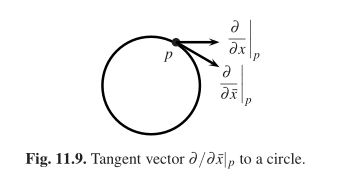
\includegraphics[scale=1]{Section11Fig11.9.png} 

\BLUE{As a reminder, the pullback is defined as
\begin{align*}
	i^*f &= f \circ i \\
	\hat{x}(p) &= (i^*x)(p) = x(i(p))= x(p) 
\end{align*}that is the $x$-coordinate of $p$
\begin{align*}
	X &= \sum \RBAR{\PART{}{\hat{x}}}_p \\
	(i_*X)(g) &= X(g\circ i) \\
	&= \sum \RBAR{\PART{g(i(x))}{\hat{x}}}_p \\
	&= \PART{g}{\hat{x}}(p)+\PART{g}{\hat{y}}(p) 
\end{align*}
}

\item Generalize (a) to a smooth curve $C$ in $\R^2$, letting $U$ be a chart in $C$ on which $\hat{x}$, the restriction of $x$ to $C$, is a local coordinate.

\end{enumerate}

\item \textbf{Critical points of a smooth map on a compact manifold}

Show that a smooth map $f$ from a compact manifold $N$ to $\R^m$ has critical point.  (\textit{Hint}: Let $\pi:\R^m \to \R$ be the projection to the first factor.  Consider the composite map $\pi \circ f: N \to \R$.  A second proof uses Corollary 11.6 adn the connectedness of $\R^m$.)

\item \textbf{Differential of an inclusion map}

On the upper hemisphere of the unit sphere $S^2$, we have the coordinate map $\phi =(u,v)$, where
\begin{align*}
	u(a,b,c)=a \AND v(a,b,c)=b.
\end{align*}So the derivations $\RBAR{\partial/\partial u}_p, \RBAR{\partial/\partial v}_p$ are tangent vectors of $S^2$ at any point $p=(a,b,c)$ on the upper hemisphere.  Let $i: S^2\to \R^3$ be the inclusion and $x,y,z$ the standard coordinates on $\R^3$.  The differential $i_*:T_pS^2\to T_p\R^3$ maps $\RBAR{\partial/\partial u}_p, \RBAR{\partial/\partial v}_p$ into $T_p\R^3$.  Thus,
\begin{align*}
	i_*\PAREN{\RBAR{\PART{}{u}}_p} &= \alpha^1\RBAR{\PART{}{x}}_p+\beta^1\RBAR{\PART{}{y}}_p+\gamma^1\RBAR{\PART{}{z}}_p,\\
	i_*\PAREN{\RBAR{\PART{}{v}}_p} &= \alpha^2\RBAR{\PART{}{x}}_p+\beta^2\RBAR{\PART{}{y}}_p+\gamma^2\RBAR{\PART{}{z}}_p,
\end{align*}for some constants $\alpha^i,\beta^i, \gamma^i$.  Find $(\alpha^i,\beta^i, \gamma^i)$ for $i=1,2$.

\item \textbf{One-to-one immersion of a compact manifold}

Prove that if $N$ is a compact manifold, then a one-to-one immersion $f:N\to M$ is an embedding.

\newcommand{\SL}{\operatorname{SL}}
\newcommand{\GL}{\operatorname{GL}}
\item \textbf{Multiplication map in $\SL(n\R)$}

Let $f: \GL(n,\R)$ be the determinant map $f(A)=\det A=\det[a_{ij}]$.  For $A \in \SL(n,\R)$, there is at least one $(k,\ell)$ such that the partial derivative $\partial f/\partial a_{k\ell}(A)$ is nonzero (Example 9.13).  Use Lemma 9.10 and the implicit function theorem to prove that
\begin{enumerate}
	\item there is a neighborhood of $A$ in $\SL(n,\R)$ in which $a_{ij}, (i,j) \ne (k,\ell)$, form a coordinate system, and $a_{k\ell}$ is a $C^\infty$ function of the other entries $a_{ij},(i,j \ne (k,\ell);$
	\item the multiplication map
	\begin{align*}
		\hat{\mu}: \SL(n,\R)\times \SL(n,\R) \to \SL(n,\R)
	\end{align*}is $C^\infty$.
\end{enumerate}

\end{enumerate}
\end{document}
